\documentclass{article}

% if you need to pass options to natbib, use, e.g.:
%     \PassOptionsToPackage{numbers, compress}{natbib}
% before loading neurips_2018

% ready for submission
% \usepackage{neurips_2018}

% to compile a preprint version, e.g., for submission to arXiv, add add the
% [preprint] option:
%     \usepackage[preprint]{neurips_2018}

% to compile a camera-ready version, add the [final] option, e.g.:
     \usepackage[final]{nips_2018}

% to avoid loading the natbib package, add option nonatbib:
%     \usepackage[nonatbib]{neurips_2018}
\usepackage[UTF8]{ctex}
\usepackage[utf8]{inputenc} % allow utf-8 input
\usepackage[T1]{fontenc}    % use 8-bit T1 fonts
\usepackage{hyperref}       % hyperlinks
\usepackage{url}            % simple URL typesetting
\usepackage{booktabs}       % professional-quality tables
\usepackage{amsfonts}       % blackboard math symbols
\usepackage{nicefrac}       % compact symbols for 1/2, etc.
\usepackage{microtype}      % microtypography

\title{Proposal}

% The \author macro works with any number of authors. There are two commands
% used to separate the names and addresses of multiple authors: \And and \AND.
%
% Using \And between authors leaves it to LaTeX to determine where to break the
% lines. Using \AND forces a line break at that point. So, if LaTeX puts 3 of 4
% authors names on the first line, and the last on the second line, try using
% \AND instead of \And before the third author name.

\author{%
%  David S.~Hippocampus\thanks{Use footnote for providing further information
%    about author (webpage, alternative address)---\emph{not} for acknowledging
%    funding agencies.} \\
%  Department of Computer Science\\
%  Cranberry-Lemon University\\
%  Pittsburgh, PA 15213 \\
%  \texttt{hippo@cs.cranberry-lemon.edu} \\
  % examples of more authors
  % \And
  % Coauthor \\
  % Affiliation \\
  % Address \\
  % \texttt{email} \\
  % \AND
  % Coauthor \\
  % Affiliation \\
  % Address \\
  % \texttt{email} \\
  % \And
  % Coauthor \\
  % Affiliation \\
  % Address \\
  % \texttt{email} \\
  % \And
  % Coauthor \\
  % Affiliation \\
  % Address \\
  % \texttt{email} \\
}

\begin{document}
% \nipsfinalcopy is no longer used

\maketitle

\section{Problem Background}
超分辨率(super-resolution, SR)问题希望从低分辨率多媒体数据重建出相应的高分辨率数据。本次比赛的场景为视频超分辨率问题,恢复降质视频本身的内容,提高视频的清晰度。


随着视频行业进入“超高清时代”,许多硬件设备已经支持超高分辨率媒体,却缺乏对应的高分辨率视频资源。视频超分辨率技术可以用来提升早期胶片或者用户自媒体视频的质量和清晰度,满足用户对于高分辨率媒体资源的需求。


超分辨率技术在图像、视频以及高维数据上均得到应用。基于深度学习的 SR 方法,主要是基于卷积神经网络(CNN)实现。在本次比赛中,处理视频数据,会存在以下挑战。


\paragraph{输出分辨率限制} 应用 CNN 的 SR 方案中,运算量会随着输出分辨率的大小而增加。
\paragraph{时序特征应用} 视频数据存在时序特征,如果同时处理多帧数据,运动可能会造成部分区域内容的剧烈变化,所以需要更加好的时序特征提取方式。
\paragraph{上采样空洞} 因为输出为高分辨率数据,所以必定会经过上采样过程。上采样过程中存在数据空洞,使用插值补齐方式无法达到很好的效果。
\paragraph{综合的评价指标} 现有的大部分方法,都是尽可能提高PSNR指标,然而由于PSNR是按像素计算的,更高的PSNR分数有可能导致感知上更大的差异。本次比赛将结合PSNR指标和VMAF指标进行综合评价,这对我们模型的选择与训练增加了挑战。

\section{Dataset Specification}
阿里巴巴优酷视频增强和超分辨率挑战赛\cite{competition}涉及1000个视频,每个视频的时间长度为4 $\sim$ 6秒。每个样本由低分辨率视频(LR)和高分辨率(HR)视频组成的视频对构成。低分辨率视频为算法的输入,高分辨率视频为增强和超分后的真值。视频数据为无压缩的y4m格式。

初赛视频250个,训练集、验证集、测试集占比为150:50:50;复赛视频750个,训练集、验证集、测试集占比为450:150:150。

复赛视频750个,训练集,验证集,测试集(A榜+B榜)分别450:150:150。

绝大部分的LR视频分辨率为480x270,HR视频为1920x1080。

\section{Evaluation Metrics}
挑战赛已经给出了视频恢复的评价指标。计算方法概括如下:
\begin{enumerate}
	\item 10\%的提交视频为完整视频结果,90\%为抽帧后的视频结果。
	\item score = PSNR指标得分$\times 80\% + $ VMAF指标得分 $\times 20\%$,其中VMAF结果为完整视频所有帧VMAF结果的均值,PSNR是所有视频中所有帧的平均值。
	\item PSNR(Peak Signal To Noise Ratio)是一种评价图像的客观标准,以dB为单位,PSNR值越大表示图像失真越小。然而,PSNR的评价结果无法与人眼看到的视觉品质完全一致。
	% 此处需要打公式
	\begin{equation}\label{key}
	PSNR = 10 \cdot \log_{10} \frac{MAX_{I}^{2}}{MSE} 
	\end{equation}
	\item VMAF(Video Multimethod Assessment Fusion) 将多种质量指标结合在一起预测主观质量。通过机器学习算法将不同指标“融合”为一个最终指标。
	
\end{enumerate}


\section{Survey}

\subsection{SRCNN}
SRCNN\cite{SRCNN}是深度学习在超分辨率领域的开山之作。通过双三次插值(见图\ref{fig:srcnn})将低分辨率图像放大成目标尺寸,然后通过三层卷积网络拟合高分辨率图像。
\begin{figure}
	\centering
	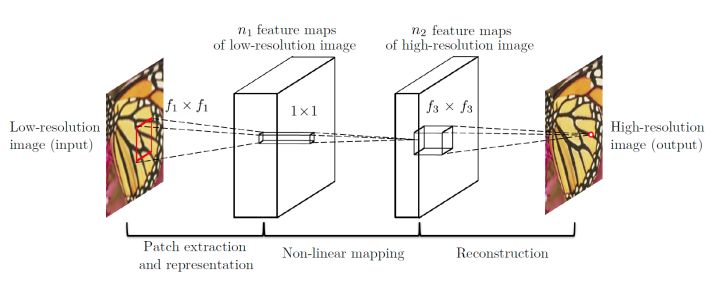
\includegraphics[width=0.8\linewidth]{SRCNN}
	\caption{}
	\label{fig:srcnn}
\end{figure}

\subsection{ESPCN}
ESPCN\cite{ESPCN}直接通过端到端的方式将低分辨率图像转换成高分辨率图像,而不需要经过插值等额外处理。具体方式见图\ref{fig:espcn},该层也被称为sub-pixel convolution layers。

设输入图像维度为1,空间大小为$H\times W$,需要放大的倍数为$r$,那么经过若干次卷积得到一个维度为$r^2$,空间大小为$H\times W$的特征图。将特征图中每个像素的$r^2$个通道排列成为$r \times r$的区域,最终得到维度为1,空间大小为$rH\times rW$的高分辨率图像。
\begin{figure}
	\centering
	\includegraphics[width=0.9\linewidth]{ESPCN}
	\caption{}
	\label{fig:espcn}
\end{figure}

\subsection{VDSR}
VDSR\cite{VDSR}的想法与残差网络相似。由于低分辨率图像和高分辨率图像的低频信息相似,因此通过只学习高频部分的残差(见图\ref{fig:vdsr})可以大大降低学习的难度,提高收敛速度。

此后SR领域的工作基本都基于图像残差进行学习。
\begin{figure}
	\centering
	\includegraphics[width=0.9\linewidth]{VDSR}
	\caption{}
	\label{fig:vdsr}
\end{figure}

\subsection{SRResnet}
SRResNet来源于SRGAN\cite{SRResNet}。图\ref{fig:srresnet}分为多个残差模块,每个残差模块内部学习图像的高频信息。在网络的最后使用sub-pixel convolution layers 来增大特征尺寸。残差的使用舍得网络的深度增加,生成的图像更加逼真。
\begin{figure}
	\centering
	\includegraphics[width=0.95\linewidth]{SRResnet}
	\caption{}
	\label{fig:srresnet}
\end{figure}

\subsection{EDSR}
EDSR\cite{EDSR}的架构非常类似SRResNet,主要的不同在于去除了其中多余的BN模块(见图\ref{fig:edsr})。BN会忽略图像特征的绝对差异,而只考虑相对差异,所以可以提高分类等高层任务的效果。但是在图像分辨率这种低层计算机视觉任务中,BN反而会破坏图像原有的对比度等信息,使得训练变慢、不稳定。

去除BN以后也可以节省计算开销,从而增加网络深度。
\begin{figure}
	\centering
	\includegraphics[width=0.8\linewidth]{EDSR}
	\caption{}
	\label{fig:edsr}
\end{figure}

\subsection{EPSR}
EPSR\cite{EPSR}在EPSR的基础上,改进了损失函数的设计。EPSR结合了MSE损失,感知损失和对抗损失,从而达到了不同指标之间的权衡。

\section{Preliminary Technical Solution }
\subsection{Model}

\subsection{Training}
\begin{itemize}
	\item 尝试不同的损失函数。例如结合MSE、感知损失、纹理匹配损失和对抗损失,并根据比赛的指标进行调整。
	\item 比赛要求不能使用额外的数据,数据增强变得非常重要。LR图像和HR图像均可用于训练,只需将图片进行目标倍率的下采样,即可得到训练的输入数据,而原图像则作为标签(\cite{ZSSR})。也可以尝试旋转、翻转等增强操作。
\end{itemize}

\section{Implementation Plan}
实现计划见表\ref{Plan}。

\begin{table}[]
	\centering
	\label{Plan}
	\begin{tabular}{|l|l|}
		\hline
		5.10-5.12 & Data preprocessing(finished)                                                                                                                                                                                                                                                  \\ \hline
		5.10-5.20 & Literature research                                                                                                                                                                                                                                                           \\ \hline
		5.15-5.24 & \begin{tabular}[c]{@{}l@{}}Read the code of EPSR and design our baseline model\\ Design and train our own model\\ Use data augmentation, learning rate strategy and \\ different loss functions to babysit our model\\ Evaluate our model based on PSNR and VMAF\end{tabular} \\ \hline
		5.25-6.18 & \begin{tabular}[c]{@{}l@{}}Preliminary contest\\ Adjust our model,do more experiments and \\ analysis the results\end{tabular}                                                                                                                                                \\ \hline
		6.19-6.25 & Hand in the final model, code and paper                                                                                                                                                                                                                                       \\ \hline
	\end{tabular}
	\caption{Implementation Plan}
\end{table}

\nocite{zhihu}
\bibliographystyle{plain}
\bibliography{proposal}
\end{document}
